\newcommand{\fgbgonedfig}{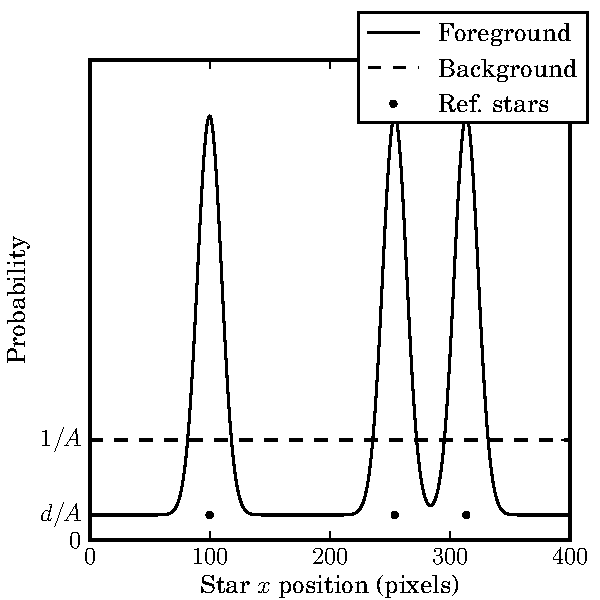
\includegraphics[width=1.000000\figunit]{fgbg-1d}}
\newcommand{\fgbgtwodfig}{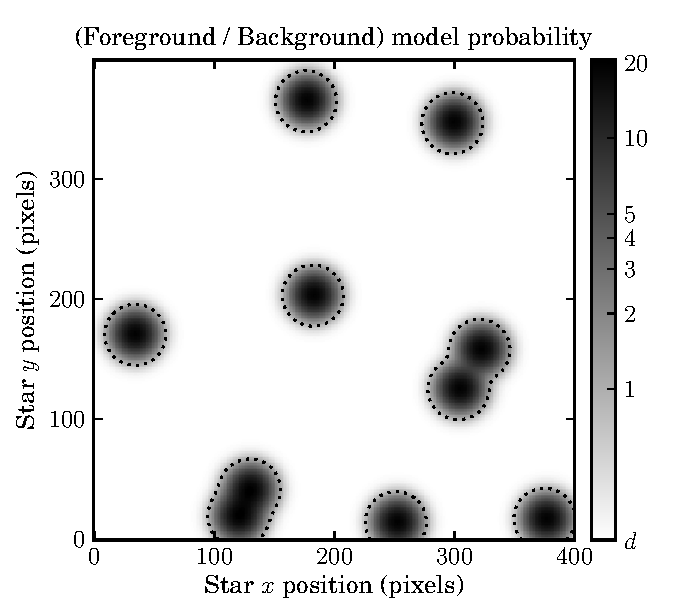
\includegraphics[width=1.150000\figunit]{fgbg-2d}}\newcommand{\symmbgfig}{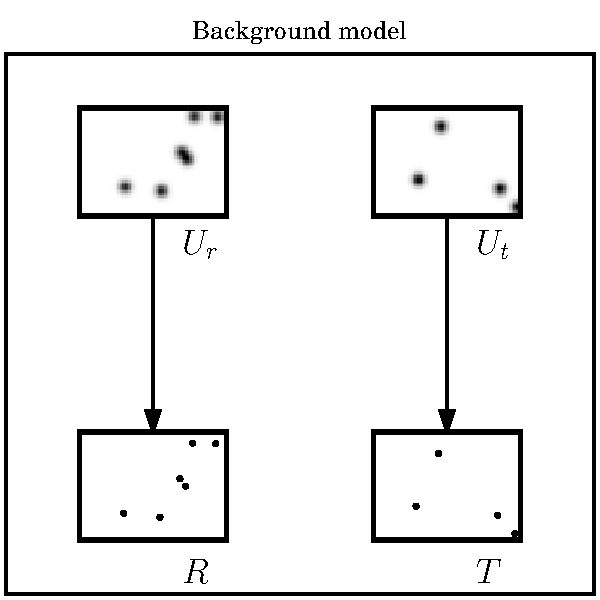
\includegraphics[width=1.000000\figunit]{symm-bg}}
\newcommand{\symmfgfig}{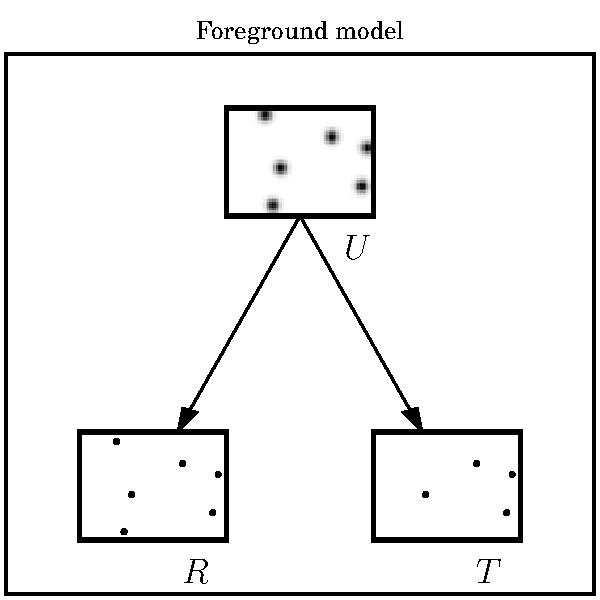
\includegraphics[width=1.000000\figunit]{symm-fg}}\newcommand{\gcreffig}{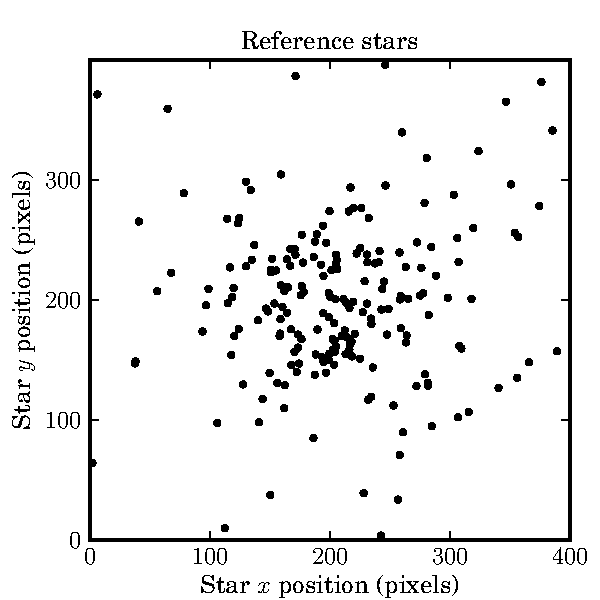
\includegraphics[width=1.000000\figunit]{gc-ref}}
\newcommand{\gctestfalsefig}{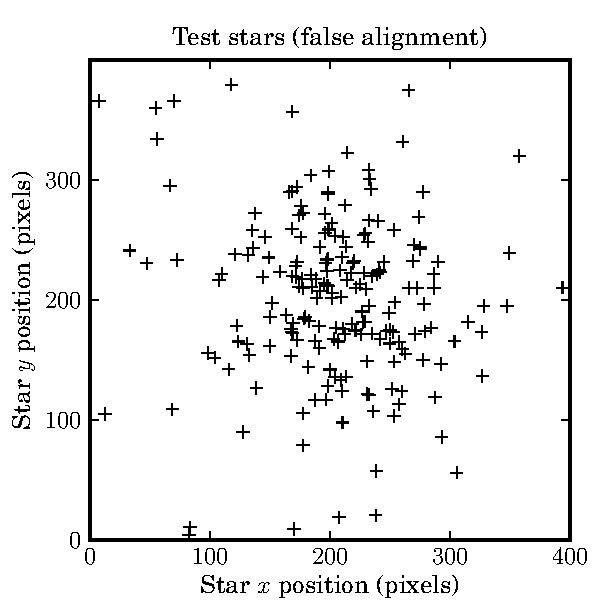
\includegraphics[width=1.000000\figunit]{gc-test-false}}
\newcommand{\gctesttruefig}{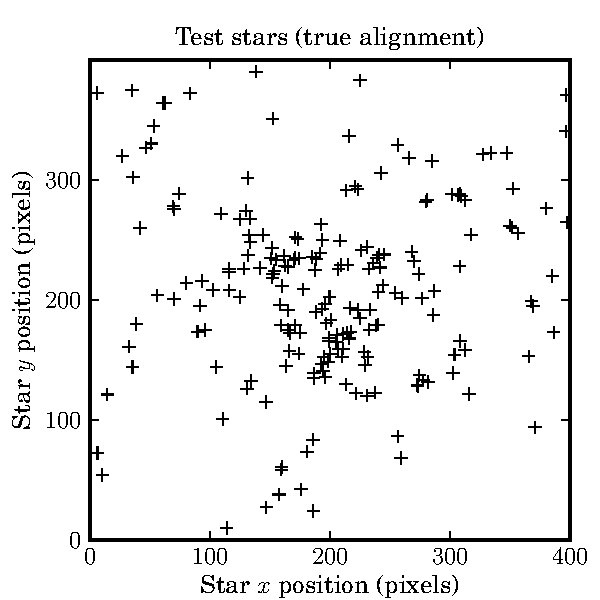
\includegraphics[width=1.000000\figunit]{gc-test-true}}
\newcommand{\gcterrainonefig}{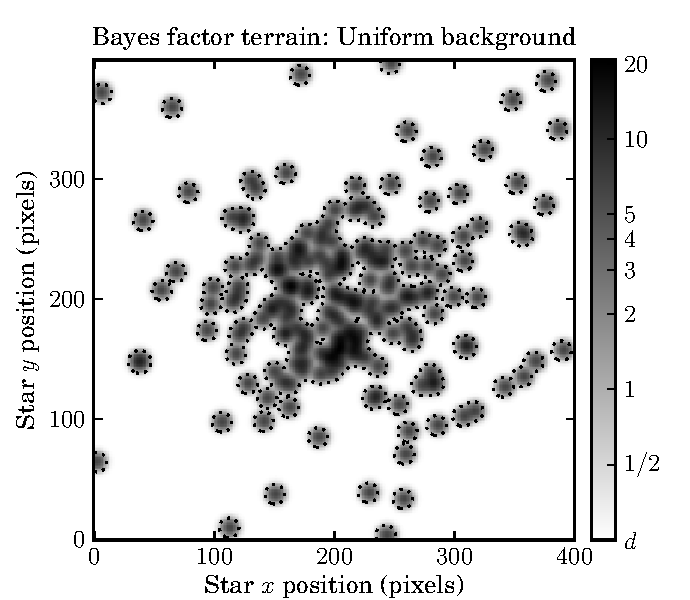
\includegraphics[width=1.150000\figunit]{gc-odds-false1}}
\newcommand{\gcterraintwofig}{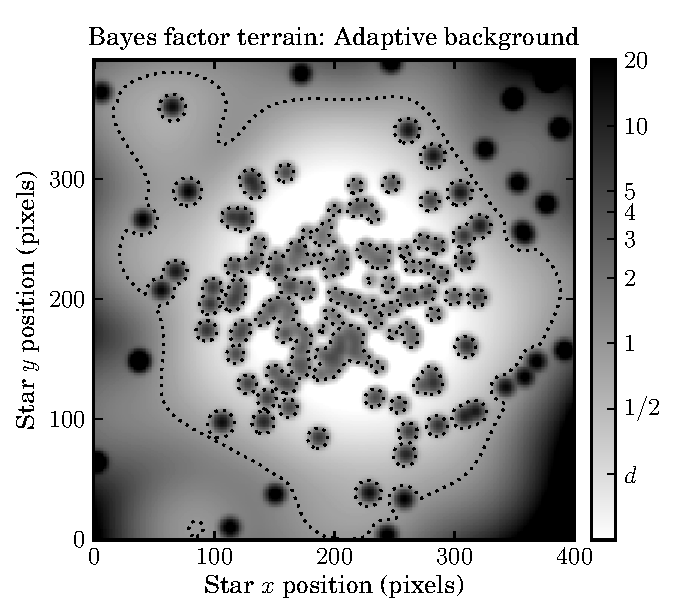
\includegraphics[width=1.150000\figunit]{gc-odds-false2}}
\newcommand{\gcbgtwofig}{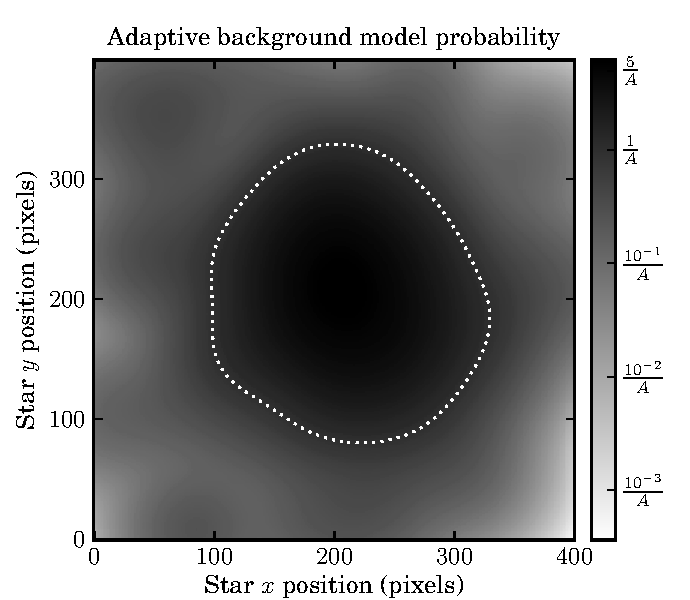
\includegraphics[width=1.150000\figunit]{gc-odds-bg}}
\newcommand{\gcbayesonefig}{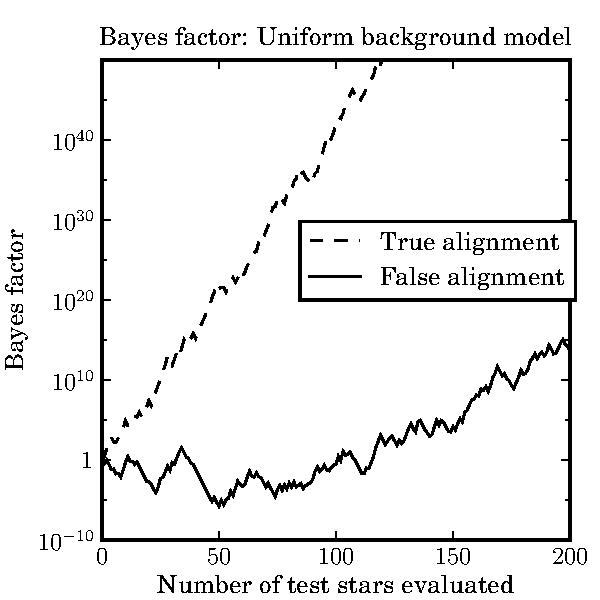
\includegraphics[width=1.000000\figunit]{gc-bayes1}}
\newcommand{\gcbayestwofig}{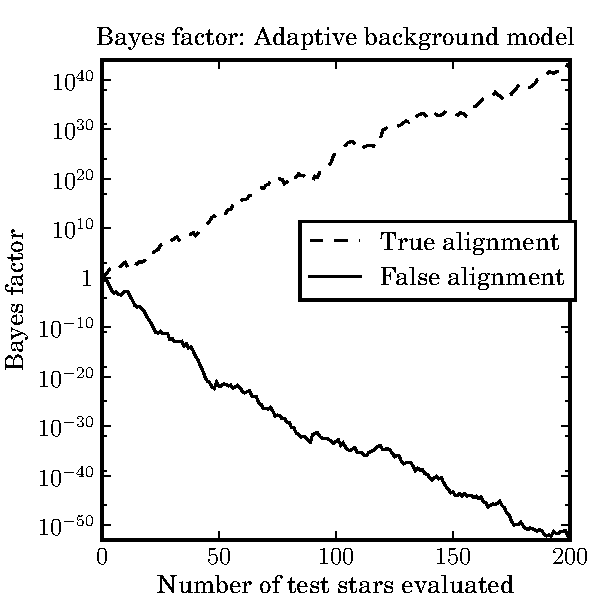
\includegraphics[width=1.000000\figunit]{gc-bayes2}}\newcommand{\nstarsfgone}{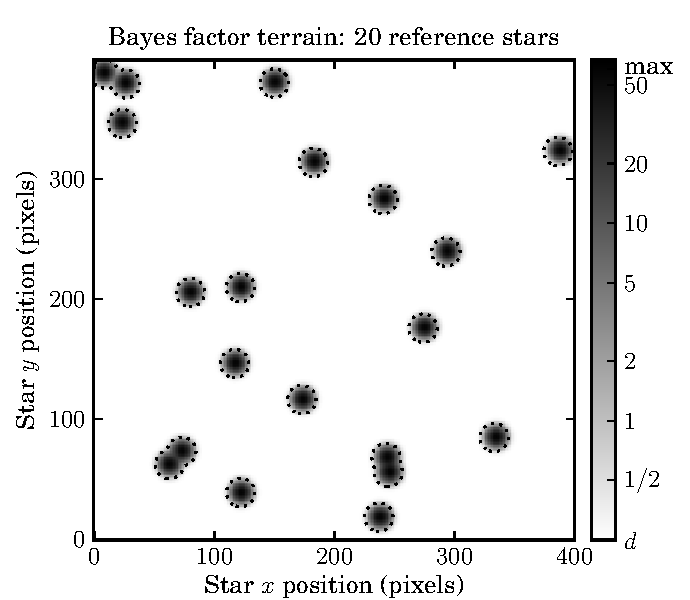
\includegraphics[width=1.150000\figunit]{nstars-fg1}}
\newcommand{\nstarsfgtwo}{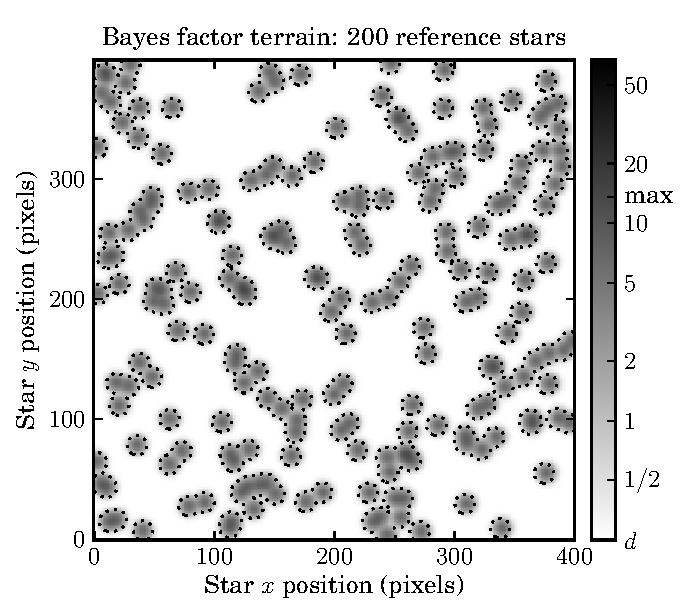
\includegraphics[width=1.150000\figunit]{nstars-fg2}}
\newcommand{\nstarsbayes}{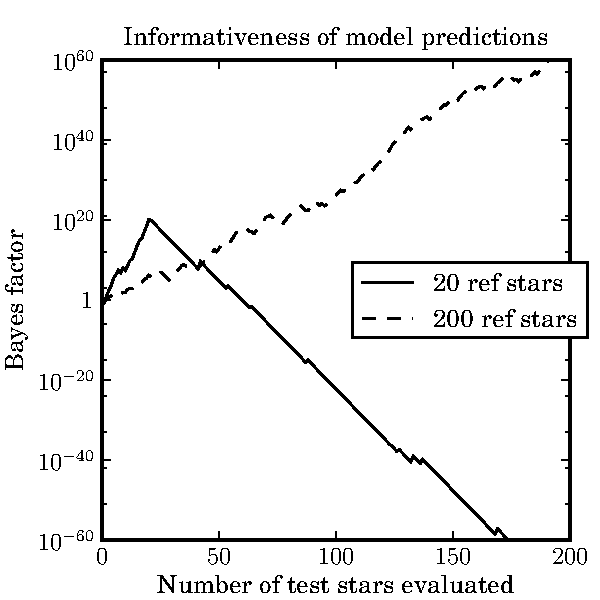
\includegraphics[width=1.000000\figunit]{nstars-bayes}}\newcommand{\exgainareafig}{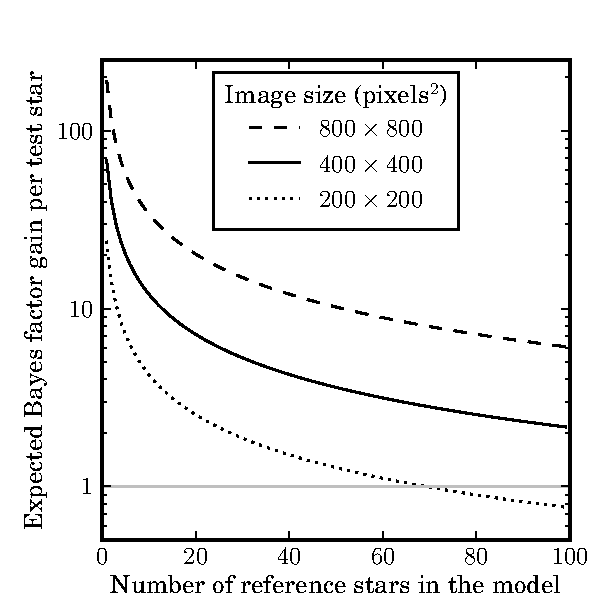
\includegraphics[width=1.000000\figunit]{exgain-1}}
\newcommand{\exgaindfig}{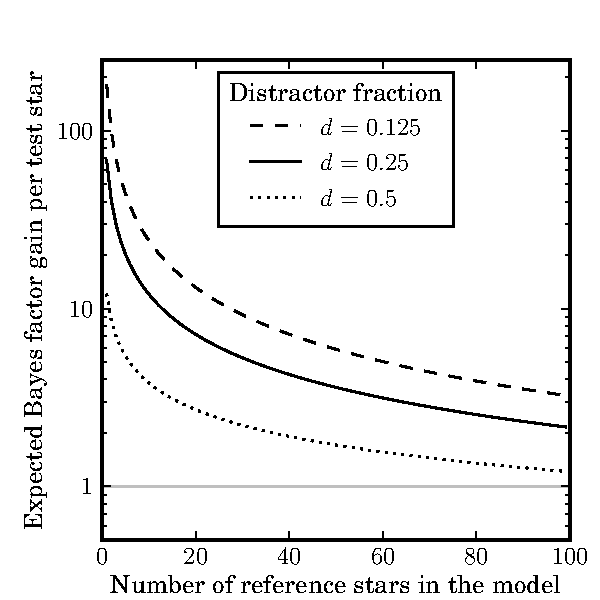
\includegraphics[width=1.000000\figunit]{exgain-2}}
\newcommand{\exgaintotalareafig}{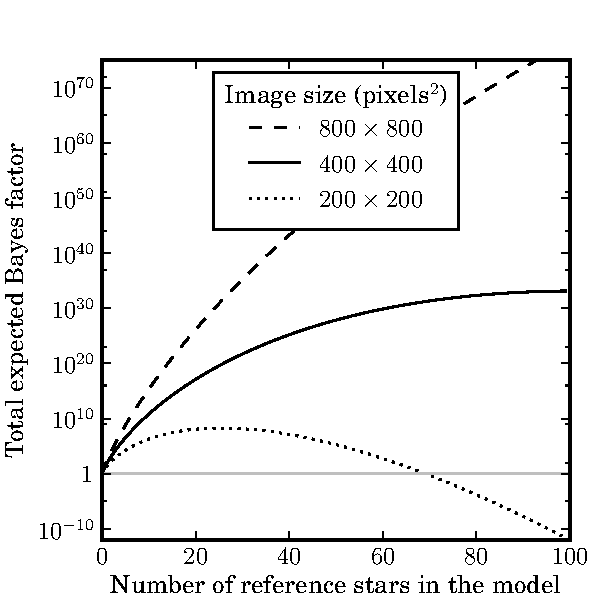
\includegraphics[width=1.000000\figunit]{exgain-total-1}}
\newcommand{\exgaintotaldfig}{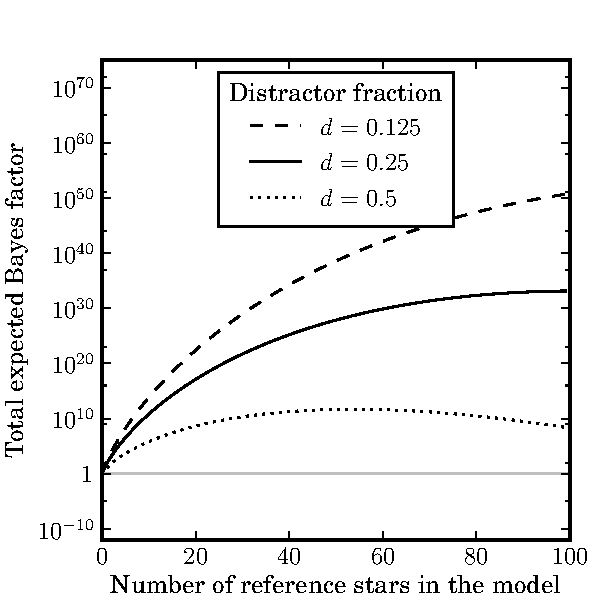
\includegraphics[width=1.000000\figunit]{exgain-total-2}}\newcommand{\donutreffig}{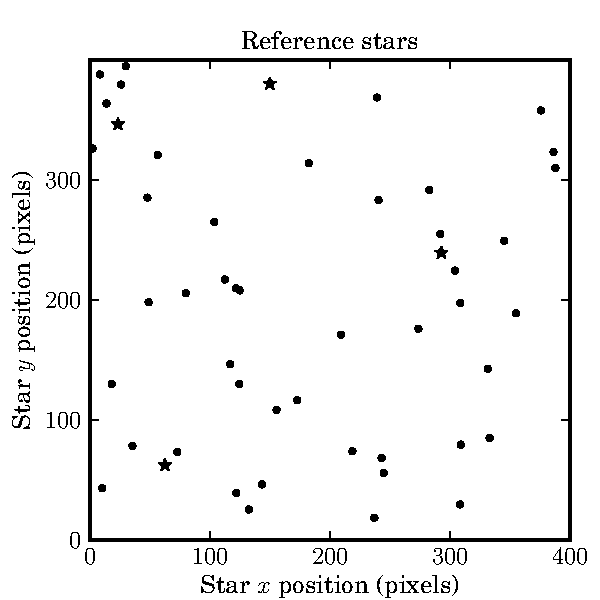
\includegraphics[width=1.000000\figunit]{donut-ref}}
\newcommand{\donuttestfig}{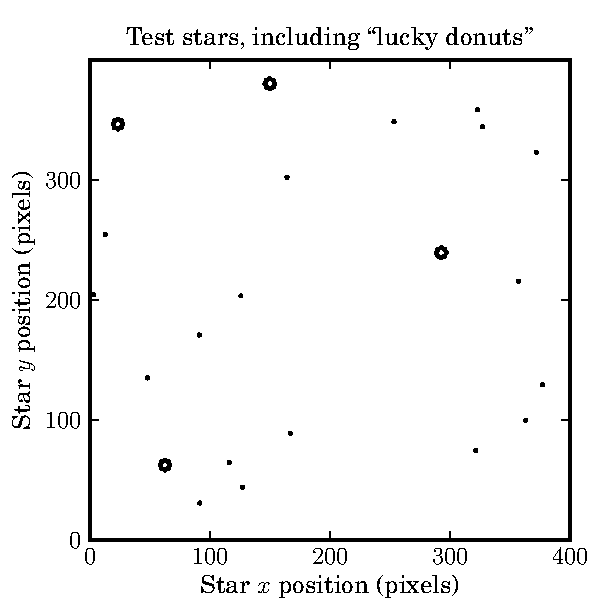
\includegraphics[width=1.000000\figunit]{donut-test}}
\newcommand{\donutbayesfig}{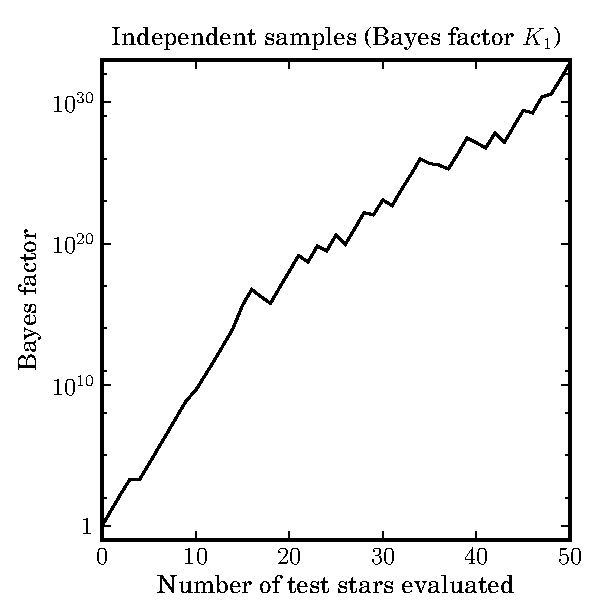
\includegraphics[width=1.000000\figunit]{donut-bayes}}
\newcommand{\donutthetasfig}{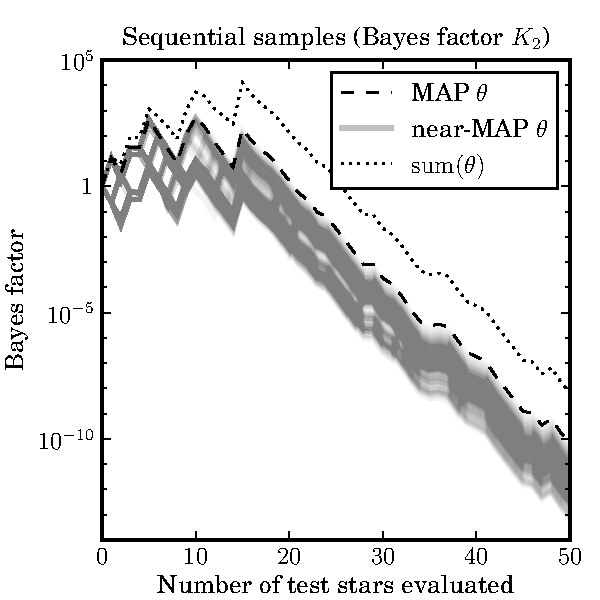
\includegraphics[width=1.000000\figunit]{donut-thetas}}\newcommand{\rorrotationfig}{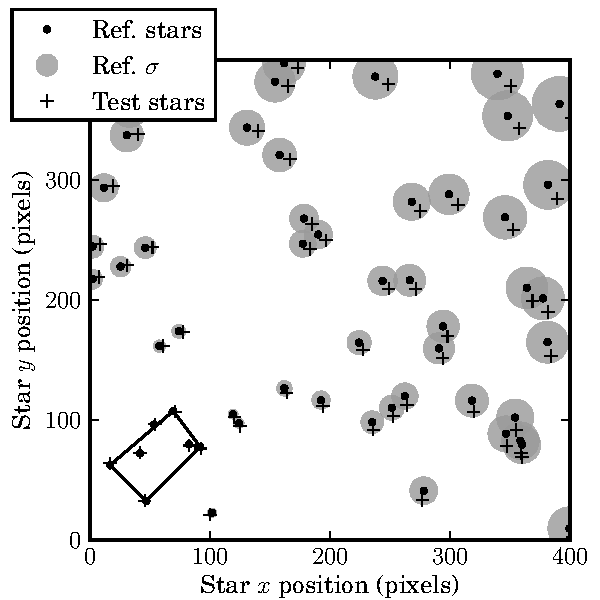
\includegraphics[width=1.000000\figunit]{ror-rotation}}
\newcommand{\rorbayesfig}{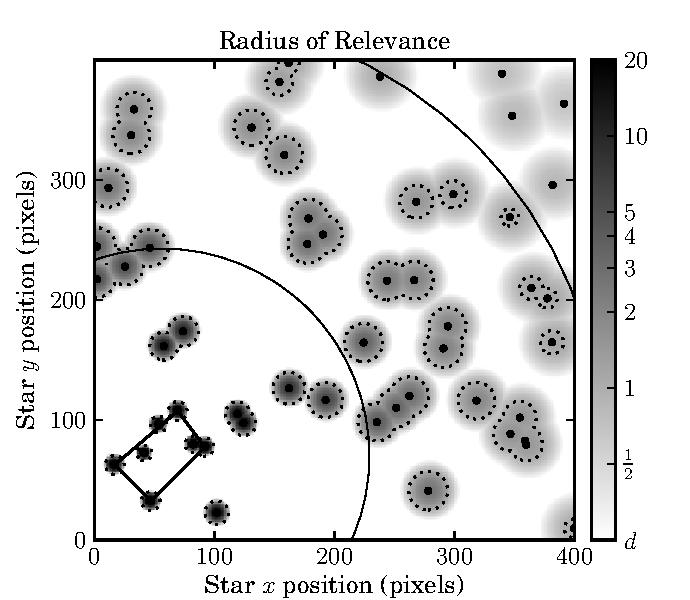
\includegraphics[width=1.150000\figunit]{ror-bayes}}
